\documentclass[a4paper]{article}

\usepackage[english]{babel}
\usepackage[utf8]{inputenc}
\usepackage{amsmath}
\usepackage{graphicx}
\usepackage[colorinlistoftodos]{todonotes}
\usepackage{makeidx}
\usepackage{setspace}
\usepackage{float}

\makeindex
\onehalfspacing
\graphicspath{ {images/}{screenshot/}}


\begin{document}

\begin{titlepage}
	\newcommand{\HRule}{\rule{\linewidth}{0.1 mm}}
	\center
	\textsc{\LARGE Università di Bologna}\\[1.5cm] % Main heading such as the name of your university/college
	
	\HRule\\[0.8 cm]
	{\huge\bfseries Relazione di tirocinio curricolare}\\[0.4cm] % Title of your document
  \HRule\\[1.5cm]
  
	\textsc{\Large Sviluppo e analisi front-end di un prodotto software con workflow
	aziendale}\\[0.3cm] % Main heading such as the name of your university/college
	\textsc{\large Presso Diennea S.R.L}\\[1.5cm] % Main heading such as the name of your university/college
	
	%------------------------------------------------
	%	Author(s)
	%------------------------------------------------
	
	\begin{minipage}{0.4\textwidth}
		\begin{flushleft}
			\large
			\textit{Autore}\\
			\textsc{Matteo Minardi}
		\end{flushleft}
	\end{minipage}
	~
	\begin{minipage}{0.4\textwidth}
		\begin{flushright}
			\large
			\textit{Tutor Aziendale}\\
			\textsc{Enrico Olivelli} % Supervisor's name
    \end{flushright}
    \begin{flushright}
			\large
			\textit{Tutor Didattico}\\
			\textsc{Annalisa Franco} % Supervisor's name
		\end{flushright}
	\end{minipage}
	

	\vfill\vfill\vfill % Position the date 3/4 down the remaining page
  
  {\large Dal \emph{18 Settembre 2017} al \emph{14 Ottobre 2017}}\\[1 cm] % Date, change the \today to a set date if you want to be precise
	
\end{titlepage}

\section{Introduzione}
\label{sec:Introduzione}

\par L'obiettivo principale di questo tirocinio curricolare era l'inserimento formativo
in un ambiente aziendale con il focus sullo sviluppo e analisi front-end per
migliorare il prodotto aziendale.\\
\par L'azienda ha sede principale a Faenza, è un'azienda di fama internazionale con 
anche una sede estera a Parigi. E' tra le aziende leader nel Digital Marketing 
orientato al Mail Marketing, ha oltre 700 clienti tra cui BMW, Stroili Oro,  Ducati,
 Findomestic e molti altri.\\
Diennea è un'azienda che lavora a stretto contatto con i clienti e la loro immagine digitale a 
trecentosessanta gradi. Da quindici anni a questa parte sviluppa un prodotto all'avanguardia
che permette al cliente di gestire tutto ciò che riguarda le campagne pubblicitarie, le newsletter e 
l'interazione digitale con i propri contatti attraverso canali come e-mail e SMS.\\
\par Il mio ruolo in tutto ciò è stato quello di far parte del team \emph{Product\&Care} con il ruolo di 
front-end developer volto a migliorare quelli che sono gli aspetti relativi alla 
veste grafica e alla \emph{UX (User Expirience)} del loro prodotto.\\
Il prodotto in questione ha nome \emph{MagNews}
\begin{figure}[H]
	
\includegraphics[width=4cm]{magnews-diennea.png}
	\centering
\end{figure}
Si occupa di gestire i clienti dell'acquirente all'interno Database su cui vengono
create campagne mirate a pubblicizzarsi nel modo più efficiente, efficace e intelligente 
possibile. Tutto questo è contornato da reportistiche dettagliate, dati in tempo reali 
e moltissime feature interessanti che lo rendono uno dei migliori prodotti in questo
campo in italia.\\ 
E' scontato precisare che per realizzare tutto questo è necessaria la combinazione
di svariate teconlogie che collaborano al fine comune di creare una piattaforma solida
scalabile e resistente allo stress esercitato dall'uso intensivo delle risorse.\\
Le risorse infatti, pur essendo di grossa portata, devono essere usate in modo
performante visto che devono servire milioni di mail ogni giorno e provvedere a centinaia
di migliaia di richieste. Per tutto questo serve un'architettura distribuita moderna e scalabile. 

Ovviamente entrando in un azienda con un alto numero di Developer è stato inevitabile
affrontare discorsi relativi al versionamento e al workflow aziendale. Tutto questo
ha concretizzato molte dinamiche viste e affrontate soltanto teoricamente durante il 
percorso accademico. 

\section{Tecnologie}
\label{sec:Tecnologie}

\section{Attività}

\section{Conclusioni}
Show a graph of the longitudinal resistivity ($\rho_{xx}$) and Hall resistivity ($\rho_{xy}$) versus magnetic field, extracted from the raw data shown in figure \ref{fig:data}. You will have the link to the data in your absalon messages, if not e-mail Guen (guen@nbi.dk). Explain how you calculated these values, and refer to the theory.

\subsection{Classical regime}
Calculate the sheet electron density $n_{s}$ and electron mobility $\mu$ from the data in the low-field regime, and refer to the theory in section \ref{sec:theory}. Explain how you retrieved the values from the data (did you use a linear fit?).
Round values off to 1 or 2 significant digits: 8.1643 ~= 8.2. Also, 5e-6 is easier to read than 0.000005.

!OBS: This part is optional (only if you have time left).
Calculate the uncertainty as follows: \newline $u(f(x, y, z)) = \sqrt{(\frac{\delta f}{\delta{x}} u(x))^{2} + (\frac{\delta f}{\delta{y}} u(y))^{2} + (\frac{\delta f}{\delta{z}} u(z))^{2}}$, where $f$ is the calculated value ($n_{s}$ or $\mu$), $x, y, z$ are the variables taken from the measurement and $u(x)$ is the uncertainty in x (and so on).

\subsection{Quantum regime}
Calculate $n_{s}$ for the high-field regime.
Show a graph of the longitudinal conductivity ($\rho_{xx}$) and Hall conductivity($\rho_{xy}$) \textbf{in units of the resistance quantum} ($\frac{h}{e^{2}}$), depicting the integer filling factors for each plateau.
Show a graph of the plateau number versus its corresponding value of $1/B$. From this you can determine the slope, which you use to calculate the electron density.
Again, calculate the uncertainty for your obtained values.

\section{Discussion 1/2-1 page}
Discuss your results. Compare the two values of $n_{s}$ that you've found in the previous section. Compare your results with literature and comment on the difference. If you didn't know the value of the resistance quantum, would you be able to deduce it from your measurements? If yes/no, why?

\newpage
\section{Some LaTeX tips}
\label{sec:latex}
\subsection{How to Include Figures}

First you have to upload the image file (JPEG, PNG or PDF) from your computer to writeLaTeX using the upload link the project menu. Then use the includegraphics command to include it in your document. Use the figure environment and the caption command to add a number and a caption to your figure. See the code for Figure \ref{fig:frog} in this section for an example.

\begin{figure}
\centering
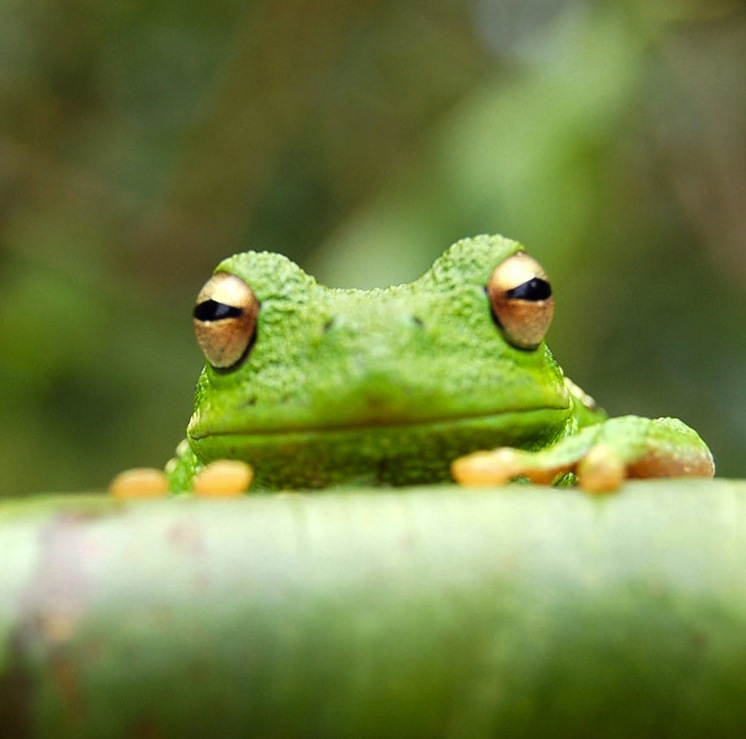
\includegraphics[width=0.3\textwidth]{frog.jpg}
\caption{\label{fig:frog}This frog was uploaded to writeLaTeX via the project menu.}
\end{figure}

\subsection{How to Make Tables}

Use the table and tabular commands for basic tables --- see Table~\ref{tab:widgets}, for example.

\begin{table}
\centering
\begin{tabular}{l|r}
Item & Quantity \\\hline
Widgets & 42 \\
Gadgets & 13
\end{tabular}
\caption{\label{tab:widgets}An example table.}
\end{table}

\subsection{How to Write Mathematics}

\LaTeX{} is great at typesetting mathematics. Let $X_1, X_2, \ldots, X_n$ be a sequence of independent and identically distributed random variables with $\text{E}[X_i] = \mu$ and $\text{Var}[X_i] = \sigma^2 < \infty$, and let

\begin{equation}
S_n = \frac{X_1 + X_2 + \cdots + X_n}{n}
      = \frac{1}{n}\sum_{i}^{n} X_i
\label{eq:sn}
\end{equation}

denote their mean. Then as $n$ approaches infinity, the random variables $\sqrt{n}(S_n - \mu)$ converge in distribution to a normal $\mathcal{N}(0, \sigma^2)$.

The equation \ref{eq:sn} is very nice.

\subsection{How to Make Sections and Subsections}

Use section and subsection commands to organize your document. \LaTeX{} handles all the formatting and numbering automatically. Use ref and label commands for cross-references.

\subsection{How to Make Lists}

You can make lists with automatic numbering \dots

\begin{enumerate}
\item Like this,
\item and like this.
\end{enumerate}
\dots or bullet points \dots
\begin{itemize}
\item Like this,
\item and like this.
\end{itemize}
\dots or with words and descriptions \dots
\begin{description}
\item[Word] Definition
\item[Concept] Explanation
\item[Idea] Text
\end{description}

We hope you find write\LaTeX\ useful, and please let us know if you have any feedback using the help menu above.

\renewcommand{\refname}{Bibliografia}
\begin{thebibliography}{9}
  \bibitem{latexcompanion} 
  Michel Goossens, Frank Mittelbach, and Alexander Samarin. 
  \textit{The \LaTeX\ Companion}. 
  Addison-Wesley, Reading, Massachusetts, 1993.
   
  \bibitem{einstein} 
  Albert Einstein. 
  \textit{Zur Elektrodynamik bewegter K{\"o}rper}. (German) 
  [\textit{On the electrodynamics of moving bodies}]. 
  Annalen der Physik, 322(10):891–921, 1905.
   
  \bibitem{knuthwebsite} 
  Knuth: Computers and Typesetting,
  \\\texttt{http://www-cs-faculty.stanford.edu/\~{}uno/abcde.html}
  \end{thebibliography}

\end{document}